\section{Hardware}

\begin{frame}{RAM}
\framesubtitle{RAM ist nur durch noch mehr RAM zu ersetzen!}
\begin{itemize}
\item 1GB für Fileserver…
\pause
\item … vergesst ZFS und btrfs
\pause
\item 2GB für Webserver…
\pause
\item …vergesst Java
\pause
\item 4GB+ für File-, Webserver und kleinen VM Host
\end{itemize}
\end{frame}

\begin{frame}{CPU}
\framesubtitle{80386 könnte ggf. eng werden.}
\begin{itemize}
\item Intel vs. AMD = Religion.
\pause
\item AES-NI = Verschlüsselung
\pause
\item 64-Bit, weil RAM
\end{itemize}
\end{frame}

\begin{frame}{Intel Core i3 vs. Atom}
\framesubtitle{Verschlüsselung}
\begin{figure}
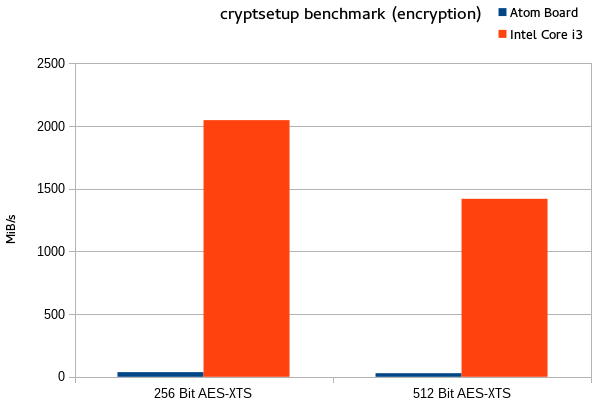
\includegraphics[width=0.8\textwidth]{images/cryptsetup-benchmark.png}
\caption{cryptsetup benchmark}
\end{figure}
\end{frame}

\begin{frame}{Intel Core i3 vs. Atom}
\framesubtitle{Kompression}
\begin{figure}
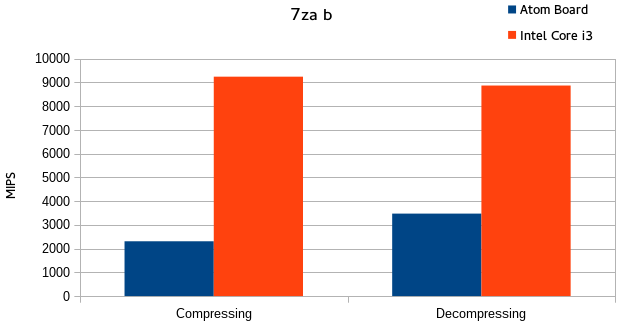
\includegraphics[width=0.8\textwidth]{images/7zab-benchmark.png}
\caption{7za b}
\end{figure}
\end{frame}

\begin{frame}{Storage}
\framesubtitle{Catcontent braucht Platz}
\begin{itemize}
\item SATA ist alternativlos
\pause
\item SSDs zu teuer
\pause
\item Backup > RAID
\pause
\item Wechselrahmen
\pause
\item RAID Levels (sinnvoll): 1, 5, 6
\pause
\item LVM
\end{itemize}
\end{frame}

\begin{frame}{Diverses}
\framesubtitle{Kleinigkeiten}
\begin{itemize}
\item Desktop Boards ohne Extras taugen
\pause
\item Stromverbrauch wird oft überschätzt
\pause
\item Netzteil nicht zu groß kaufen
\end{itemize}
\end{frame}
